\newpage
\subsection{Caso d'uso UC2:  Main post-autenticazione }
\label{UC2}
\begin{figure}[ht]
	\centering
	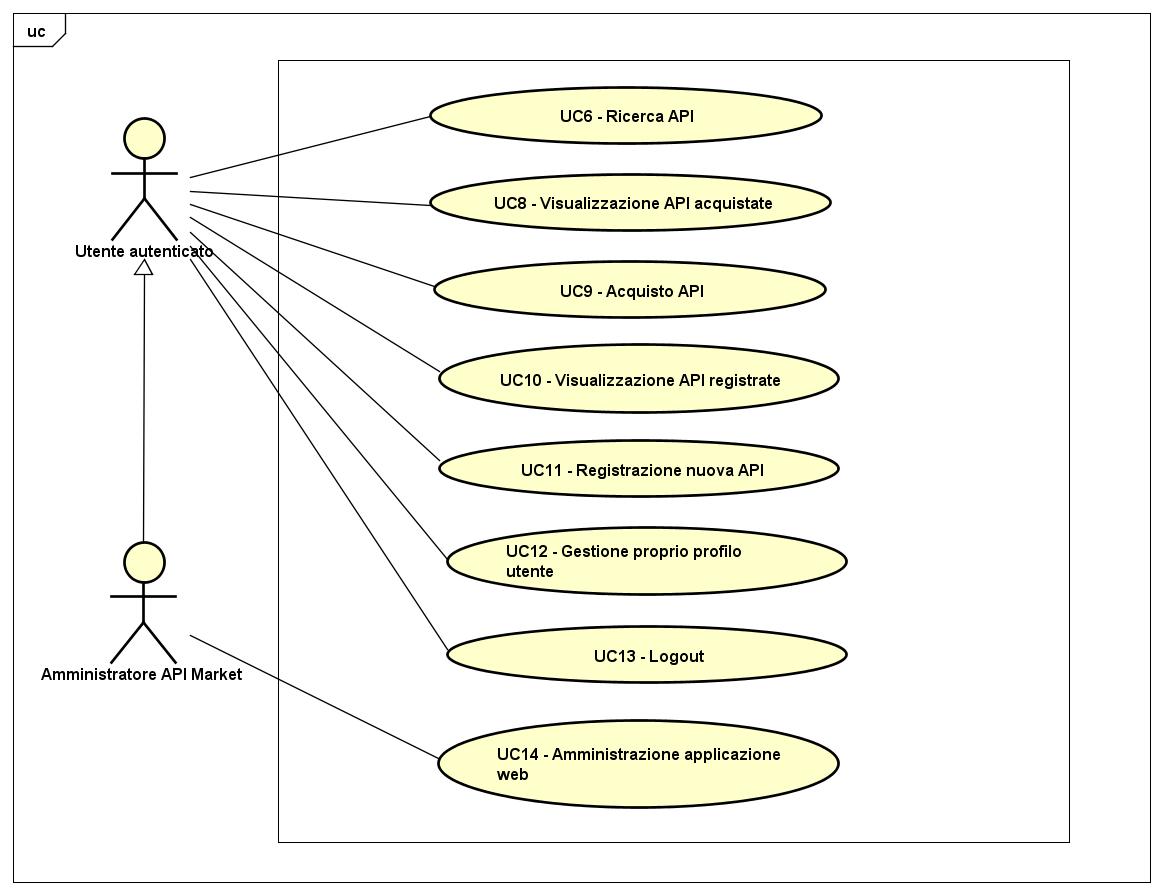
\includegraphics[scale=0.45]{UML/UC2.png}
	\caption{UC2: Main post-autenticazione}
\end{figure}

\begin{longtable}{ l | p{11cm}}
	\hline
	\rowcolor{Gray}
	 \multicolumn{2}{c}{UC2 - Main post-autenticazione} \\
	 \hline
	\textbf{Attori} & Utente autenticato, Amministratore API Market \\
	\textbf{Descrizione} & L'attore tramite la schermata principale
	dell'applicazione, può accedere e sfruttare le funzionalità a lui disponibili: l'interazione
	con il proprio profilo utente, con le API non acquistate e non, con le API registrate, la
	registrazione di una nuova API, il logout. 
	L'Amministratore API Market, oltre alle funzionalità offerte all'utente autenticato, può
	visualizzare i dati di utilizzo delle API ed amministrare l'applicazione web.  \\
	\textbf{Pre-Condizioni} & L'attore ha avviato l'applicazione web e si è autenticato \\
	\textbf{Post-Condizioni} & L'applicazione ha eseguito le richieste dell'attore \\
	\textbf{Scenario Principale} & 
	\begin{enumerate*}[label=(\arabic*.),itemjoin={\newline}]
		\item L'attore può interagire con il proprio profilo utente
		\item L'attore può interagire con le API da lui non acquistate
		\item L'attore può interagire con le API da lui acquistate
		\item L'attore può interagire con le API da lui registrate
		\item L'attore può registrare una nuova API
		\item L'attore può effettuare il logout
		\item L'attore Amministratore API Market può visualizzare i dati di utilizzo delle singole API 
		\item L'attore Amministratore API Market può amministrare l'applicazione web
	\end{enumerate*}\\
\end{longtable}